\begin{frame}
    \frametitle{Problem 3.11}

    \textbf{Problem. } Let \(M\) be a smooth manifold. Show that the tensor product over \(C(M)\)
    of two projective \(C(M)\)-modules is again a projective \(C(M)\)-module.

    % I prove this specifically for C(M) modules using ideas from vector
    % bundles, painfully, and we'll see in a bit how this is proved in a larger
    % context for an arbitrary ring with Vatsal in Q12.

\end{frame}

\begin{frame}
    \frametitle{Reframing}

    Let \(M\) be a smooth manifold. Show that the tensor product over \(C(M)\)
    of two \textcolor{red}{spaces of smooth sections} over vector bundles is
    again a \textcolor{red}{space of sections} over a vector bundle. \\ \pause

    For each pair of vector bundles \(E_1, E_2\), \(\exists E \in
    \textsf{Bundle}_M\) such that 
    
    \begin{gather*}        
        \Gamma(E_1) \otimes_{C(M)} \Gamma(E_2) \cong \Gamma(E)~.
    \end{gather*}

    % add swan theorem

    % clarify tensor product of vector bundles

\end{frame}

\begin{frame}

    We propose that \(E = E_1\otimes E_2\). \pause

    Suppose we have a map between the two spaces, \(\chi\). We show that it is
    bijective. \pause

    If \(E_1, E_2\) are trivial bundles of rank \(k_1, k_2\) respectively, we
    can construct a linearly independent basis of sections for each
    \(\Gamma(E_i)\). Let a choice of such bases be given by \(\{a_i\}\) and
    \(\{b_i\}\). These are frame fields for the individual bundles. \\ \pause

    Elements in the space \(\Gamma(E_1) \otimes \Gamma(E_2)\) are tensor
    products of sections \(s_1 \otimes s_2\), defined as mapping any point \(p
    \in M\) to \(s_1(p)\otimes s_2(p) \in E_{1p} \otimes E_{2p}\). \\ \pause

    \(\chi\) maps this to itself in the RHS. \(\chi\) is injective as an
    inclusion map.

    % Set here, E to be a trivial bundle of rank higher than the max rank of E_1

\end{frame}

\begin{frame}
    \frametitle{Surjectivity}

    % is problematic, the sections on a tensor product of an arbitrary bundle
    % may be horrendous, begin with trivial bundles

    The tensor product \(\{a_i\} \otimes \{b_i\}\) produces a frame field for
    \(\Gamma(E)\). Since this field is trivial, its frame field has exactly the
    same dimension as its rank.

    % specify that ai and bi are frame fields

    % we can argue using the fact that the rank of the bundle carries over as
    % the dimension of the space of sections

    % so it is clear in the case E1 E2 are trivial. What happens when they are
    % not? Can we forcefully trivialise them?

\end{frame}

\begin{frame}
    \frametitle{Trivialising Bundles}

    \begin{theorem}[Whitney Summands of Trivial Vector Bundles]
        If \(X\) is a paracompact Hausdorff space, and \(E \to X\) is a
        topological vector bundle, then for every vector subbundle \(E_1
        \hookrightarrow E\), there exists a direct summand \(E_2 \hookrightarrow
        E\) such that 

        \begin{gather*}
            E_1 \oplus E_2 \cong E~.
        \end{gather*}

    \end{theorem}

    % choose E to be a trivial bundle larger than E1

\end{frame}

\begin{frame}

    Consider trivialisations of the chosen bundles \(E_1 \oplus E_1^\bot\) and
    \(E_2 \oplus E_2^\bot\). We can then construct the diagram

    \begin{center}
        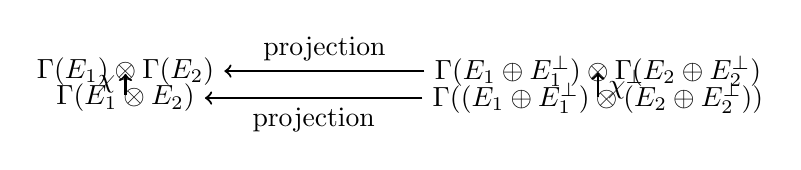
\begin{tikzpicture}[node distance={6cm}, thick, main/.style = {draw=none}]
            \node[main] (1)                         {\(\Gamma(E_1) \otimes \Gamma(E_2)\)};
            \node[main] (2) [right of=1]            {\(\Gamma(E_1\oplus E_1^\bot) \otimes \Gamma(E_2\oplus E_2^\bot)\)};
            \node[main] (3) [below=1]               {\(\Gamma(E_1\otimes E_2)\)};
            \node[main] (4) [right of=3]            {\(\Gamma((E_1\oplus E_1^\bot) \otimes (E_2\oplus E_2^\bot))\)};
            
            \draw[->] (2) to node[midway, above] {projection} (1);
            \draw[->] (1) to node[midway, left] {\(\chi\)} (3);
            \draw[->] (2) to node[midway, right] {\(\chi^\bot\)} (4);
            \draw[->] (4) to node[midway, below] {projection} (3);
        \end{tikzpicture}
    \end{center}

    The diagram commutes. All the other arrows are known to be surjective, the
    surjectivity of \(\chi\) follows.

\end{frame}

\begin{frame}

    Similarly, for the injectivity, we have the diagram with flipped arrows

    \begin{center}
        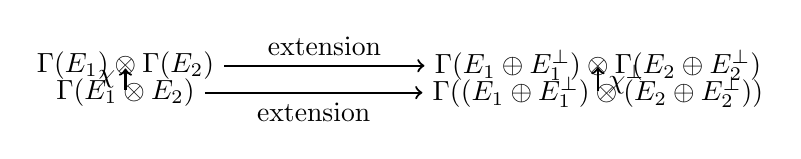
\begin{tikzpicture}[node distance={6cm}, thick, main/.style = {draw=none}]
            \node[main] (1)                         {\(\Gamma(E_1) \otimes \Gamma(E_2)\)};
            \node[main] (2) [right of=1]            {\(\Gamma(E_1\oplus E_1^\bot) \otimes \Gamma(E_2\oplus E_2^\bot)\)};
            \node[main] (3) [below=1]               {\(\Gamma(E_1\otimes E_2)\)};
            \node[main] (4) [right of=3]            {\(\Gamma((E_1\oplus E_1^\bot) \otimes (E_2\oplus E_2^\bot))\)};
            
            \draw[->] (1) to node[midway, above] {extension} (2);
            \draw[->] (1) to node[midway, left] {\(\chi\)} (3);
            \draw[->] (2) to node[midway, right] {\(\chi^\bot\)} (4);
            \draw[->] (3) to node[midway, below] {extension} (4);
        \end{tikzpicture}
    \end{center}

    The extension maps take an element to its copy in the codomain with padded
    zeroes (when viewed as a vector).

    The diagram commutes. All the other arrows are known to be surjective, the
    surjectivity of \(\chi\) follows.

\end{frame}

\begin{frame}

    The diagram for an object in each space

    \begin{center}
        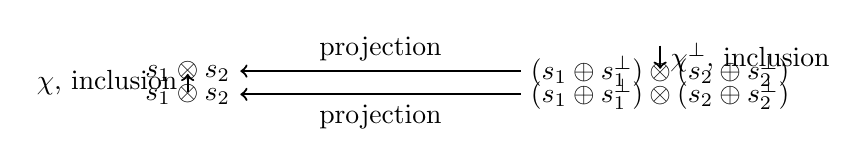
\begin{tikzpicture}[node distance={6cm}, thick, main/.style = {draw=none}]
            \node[main] (1)                         {\(s_1 \otimes s_2\)};
            \node[main] (2) [right of=1]            {\((s_1 \oplus s_1^\bot) \otimes (s_2 \oplus s_2^\bot)\)};
            \node[main] (3) [below=1]               {\(s_1\otimes s_2\)};
            \node[main] (4) [right of=3]            {\((s_1 \oplus s_1^\bot) \otimes (s_2 \oplus s_2^\bot)\)};
            
            \draw[->] (2) to node[midway, above] {projection} (1);
            \draw[->] (1) to node[midway, left] {\(\chi\), inclusion} (3);
            \draw[->] (2) to node[midway, right] {\(\chi^\bot\), inclusion} (4);
            \draw[->] (4) to node[midway, below] {projection} (3);
        \end{tikzpicture}
    \end{center}

\end{frame}

\begin{frame}

    Finally, since \(\chi\) is injective and surjective, it gives an isomorphism
    between \(\Gamma(E_1) \otimes\Gamma(E_2)\) and \(\Gamma(E_1 \otimes E_2)\)
    as required.

    % making the tensor product of the two spaces of sections another space of
    % sections, reframing again, making the tensor product of two projective
    % C(M) modules again a projective C(M) module.

\end{frame}